\documentclass[a4paper,12pt]{article}

\usepackage[margin=1.0in]{geometry}
\usepackage{fancyhdr}
\usepackage{lastpage}
\usepackage{url, lipsum}
\usepackage{tabularx}
\usepackage{graphicx}

\usepackage{natbib}

\usepackage[nottoc]{tocbibind}
\usepackage[english]{babel}
\usepackage[utf8]{inputenc}


\newcommand{\HRule}[1]{\rule{\linewidth}{#1}}
%\setcounter{tocdepth}{1}
%\setcounter{secnumdepth}{5}
\graphicspath{/images/}

%-------------------------------------------------------------------------------
% HEADER & FOOTER
%-------------------------------------------------------------------------------
\pagestyle{fancy}
\fancyhf{}
\setlength\headheight{15pt}
\fancyhead[L]{Henry Senior }
\fancyhead[R]{Student ID: @00454779}
\fancyfoot[R]{Page \thepage\ of \pageref{LastPage}}

%-------------------------------------------------------------------------------
% TITLE PAGE
%-------------------------------------------------------------------------------
\begin{document}
	
	\title{ \normalsize \textsc{Software Projects with Agile Techniques}
		\\ [2.0cm]
		\HRule{0.5pt} \\
		\LARGE \textbf{\uppercase{Semester One Assessment 1}}
		\HRule{2pt} \\ [0.5cm]}
	
	\date{6th December, 2017}
	
	\author{
		Henry Senior \\ \\
		Student ID: @00454779 \\ 
		Username: STC765 \\
		CRN: 34129
	}
	
\maketitle
\newpage

\section*{Executive Summary}
\addcontentsline{toc}{section}{Executive Summary}
The aim of this report was to model a given system using the industry standard Universal Modelling Language (UML) notation. Outlined in the report are all the Use Cases of the system (including Textual Use Cases), a Static Model of the system, and two Activity Diagrams which show in detail the sequences taken in certain Use Cases. The report highlights how UML provides different approaches to modelling the system. It also details how different methods may be more applicable that others depending on which aspect of the system is being modelled. 

\tableofcontents
\newpage
\section{Introduction}
TODO
\newpage
\section{Use Cases}
When modelling a system, it is important to understand how different actors may interact with the system. This kind of interaction is best shown through Use Case diagrams, with details of the interactions being shown in Textual Use Cases.

\subsection{Use Case Diagram}
\begin{center}
	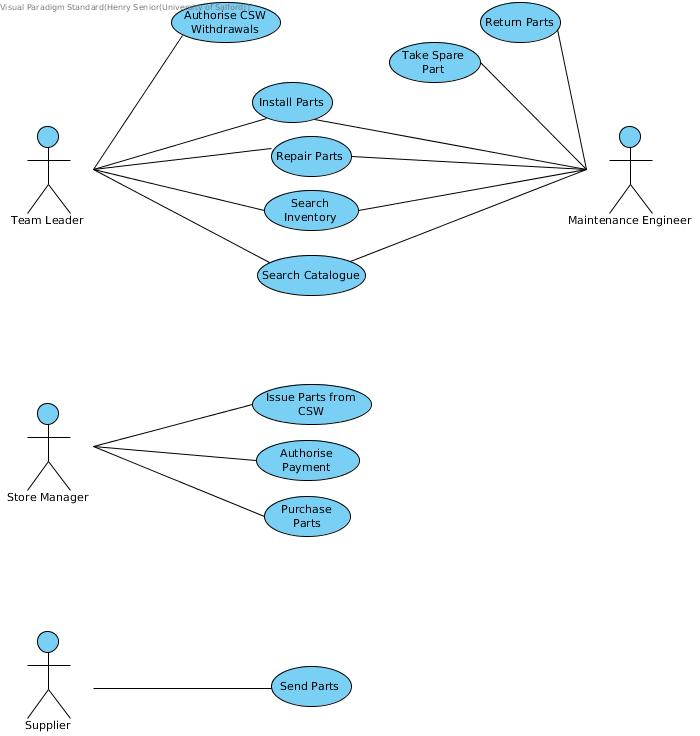
\includegraphics[width=\textwidth]{images/Use-Case.jpg}
\end{center}

\newpage

\subsection{Textual Use Cases}
\begin{table}[h]
	\centering
	\caption{Search Inventory}
	\label{Search-Inventory}
	\begin{tabularx}{\textwidth}{| l | X |}
		\hline
		Use Case Title	&  Search Inventory\\ \hline \hline
		Primary Actor	&  Team Leader or Maintenance Engineer \\ \hline
		Goal	&  Search the CSW for parts\\ \hline
		Scope	&  Central Storage Warehouse Web-based System\\ \hline
		Preconditions	&  The Team Leader or Maintenance Engineer needs to replace a part\\ \hline
		Postconditions	&  The Team Leader or Maintenance Engineer will know whether or not the part is currently in the CSW\\ \hline
		Main Success Scenario	&  
		1) The Team Leader or Maintenance Engineer searches for an item using the CSW \newline
		2) The Team Leader or Maintenance Engineer finds the part they are searching for
		\\ \hline
		Extensions	&  2a) The Team Leader or Maintenance Engineer cannot find the part they are after \\ \hline
	\end{tabularx}
\end{table}

\begin{table}[h]
	\centering
	\caption{Search Catalogue}
	\label{Search-Catalogue}
	\begin{tabularx}{\textwidth}{| l | X |}
		\hline
		Use Case Title	&  Search Catalogue\\ \hline \hline
		Primary Actor	&  Team Leader or Maintenance Engineer \\ \hline
		Goal	&  Search the Catalogue for parts not in the CSW\\ \hline
		Scope	&  Central Storage Warehouse Web-based System\\ \hline
		Preconditions	&  The Team Leader or Maintenance Engineer needs to replace a part but the part is not in the CSW\\ \hline
		Postconditions	&  The Team Leader or Maintenance Engineer will know whether or not they can order the part\\ \hline
		Main Success Scenario	&  
		1) The Team Leader or Maintenance Engineer searches for an item using the CSW Catalogue \newline
		2) The Team Leader or Maintenance Engineer finds the part they are searching for
		\\ \hline
		Extensions	&  2a) The catalogue does not contain the item the Team Leader or Maintenance Engineer desires \\ \hline
	\end{tabularx}
\end{table}

\begin{table}[]
	\centering
	\caption{Install Parts}
	\label{Install-Parts}
	\begin{tabularx}{\textwidth}{| l | X |}
		\hline
		Use Case Title	&  Install Parts\\ \hline \hline
		Primary Actor	&  Team Leader or Maintenance Engineer \\ \hline
		Goal	&  Install new parts in the plant\\ \hline
		Scope	&  Gas Turbine Power Station\\ \hline
		Preconditions	&  A need to install a new part\\ \hline
		Postconditions	&  The new part will have been installed\\ \hline
		Main Success Scenario	&  
		1) The Team Leader or Maintenance Engineer will search for the item in the CSW \newline
		2) They will withdraw the item from the CSW \newline
		3) They will install the new part \newline
		4) The old part will be returned to the CSW for refurbishment or be disposed as scrap 
		\\ \hline
		Extensions	&  2a) The part is not in the CSW \newline 2b) The part has a value of over \pounds$50,000$, so they will have to gain authorisation from a Team Leader \\ \hline
	\end{tabularx}
\end{table}

\begin{table}[]
	\centering
	\caption{Repair Parts}
	\label{Repair-Parts}
	\begin{tabularx}{\textwidth}{| l | X |}
		\hline
		Use Case Title	&  Repair Parts\\ \hline \hline
		Primary Actor	&  Team Leader or Maintenance Engineer\\ \hline
		Goal	&  Repair faulty parts within the power station\\ \hline
		Scope	&  Gas Turbine Power Station \\ \hline
		Preconditions	&  A part within the power station needs to be replaced \\ \hline
		Postconditions	&  The faulty part will be replaced \\ \hline
		Main Success Scenario	&  
		1) They will repair the part
		\\ \hline
		Extensions	&  The part cannot be repaired \\ \hline
	\end{tabularx}
\end{table}

\begin{table}[]
	\centering
	\caption{Take Spare Parts}
	\label{Take-Spare-Parts}
	\begin{tabularx}{\textwidth}{| l | X |}
		\hline
		Use Case Title	&  Take Spare Parts\\ \hline \hline
		Primary Actor	&  Maintenance Engineer\\ \hline
		Goal	&  Allow the maintenance engineer to withdraw parts from the CSW with values less than \pounds$50,000$\\ \hline
		Scope	&  Central Storage Warehouse Web-Based System\\ \hline
		Preconditions	&  A part in the power station needs to be replaced or installed\\ \hline
		Postconditions	&  The new part has been successfully installed \\ \hline
		Main Success Scenario	&  
		1) A part needs replacing or installing \newline
		2) The Maintenance Engineer searches for the part in the CSW \newline
		3) The Maintenance Engineer can withdraw the part
		\\ \hline
		Extensions	&  2a) The part is not in the CSW \newline 3a) The part has a value of over \pounds$50,000$ so the Maintenance Engineer needs to gain authorisation from a Team Leader \\ \hline
	\end{tabularx}
\end{table}

\begin{table}[]
	\centering
	\caption{Return Parts}
	\label{Return-Parts}
	\begin{tabularx}{\textwidth}{| l | X |}
		\hline
		Use Case Title	&  Return Parts\\ \hline \hline
		Primary Actor	&  Maintenance Engineer\\ \hline
		Goal	&  To return a part back into the CSW\\ \hline
		Scope	&  Central Storage Warehouse\\ \hline
		Preconditions	&  The part is no longer required, or there is not enough time left to install it\\ \hline
		Postconditions	&  The part is now stored in the CSW\\ \hline
		Main Success Scenario	& 
		1) The part is no longer going to be used \newline
		2) The part is signed back into the CSW
		\\ \hline
		Extensions	&  2a) The part cannot be signed back into the CSW \\ \hline
	\end{tabularx}
\end{table}

\begin{table}[]
	\centering
	\caption{Authorise CSW Withdrawals}
	\label{Authorise-CSW-Withdrawals}
	\begin{tabularx}{\textwidth}{| l | X |}
		\hline
	Use Case Title	&  Authorise CSW Withdrawals\\ \hline \hline
	Primary Actor	&  Team Leader\\ \hline
	Goal	&  Authorise the withdrawals of spare parts in the CSW of cost greater than \pounds$50,000$\\ \hline
	Scope	&  Central Storage Warehouse Web Based System\\ \hline
	Preconditions	&  A maintenance engineer must want to withdraw a part that is greater than \pounds$50,000$ in value.\\ \hline
	Postconditions	&  The part can be issued by the store manager.\\ \hline
	Main Success Scenario	&  
		1) A maintenance engineer searches for a part in the CSW \newline
		2) The part is in the CSW \newline
		3) The desired part has a value of over \pounds$50,000$ \newline
		4) The maintenance engineer asks the team leader to authorise the withdrawal \newline
		5)The team leader authorises the withdrawals
	\\ \hline
	Extensions	&  2a) The part is not in the CSW \newline
	5a) The team leader does not authorise the withdrawal \\ \hline
	\end{tabularx}
\end{table}

\begin{table}[]
	\centering
	\caption{Issue Parts}
	\label{Issue Parts}
	\begin{tabularx}{\textwidth}{| l | X |}
		\hline
		Use Case Title	&  Issue Parts \\ \hline \hline
		Primary Actor	&  Store Manager \\ \hline
		Goal	&  Issue parts from the CSW to the person requesting the parts\\ \hline
		Scope	&  Central Storage Warehouse\\ \hline
		Preconditions	&  A withdraw request must be made\\ \hline
		Postconditions	&  The item is withdrawn from the CSW \\ \hline
		Main Success Scenario	&  
			1) A Team Leader or Maintenance Engineer requests a part from the CSW \newline
			2) The Store Manager issues the part to them
		\\ \hline
		Extensions	& 2a) The Store Manager does not issue the part \\ \hline
	\end{tabularx}
\end{table}

\begin{table}[]
	\centering
	\caption{Purchase Parts}
	\label{Purchase-Parts}
	\begin{tabularx}{\textwidth}{| l | X |}
		\hline
		Use Case Title	&  Purchase Parts\\ \hline \hline
		Primary Actor	&  Store Manager \\ \hline
		Goal	&  To refill stock in the CSW by purchasing parts from the Supplier\\ \hline
		Scope	&  Central Storage Warehouse and Financial Management System (FMS)\\ \hline
		Preconditions	&  Store Manager has received a requisition\\ \hline
		Postconditions	&  The required goods are received \\ \hline
		Main Success Scenario	& 
		1) A purchase order is created \newline
		2) The purchase order is sent to the Supplier \newline
		3) The Supplier sends the Store Manager the goods, along with an invoice 
		\\ \hline
		Extensions	& 
		2a) The purchase order is not sent to the Supplier \newline
		3a) Goods and/or an invoice are not sent to the Store Manager  
		\\ \hline
	\end{tabularx}
\end{table}

\begin{table}[]
	\centering
	\caption{Authorise Payments}
	\label{Authorise Payments}
	\begin{tabularx}{\textwidth}{| l | X |}
		\hline
		Use Case Title	&  Authorise Payments \\ \hline \hline
		Primary Actor	&  Store Manager \\ \hline
		Goal	&  Authorise the payments of legitimate invoices sent from suppliers\\ \hline
		Scope	&  Power Station Financial Management System \\ \hline
		Preconditions	&  A part has been purchased and the part and it's invoice have been delivered to the CSW\\ \hline
		Postconditions	&  The invoice is deemed legitimate and is therefore paid \\ \hline
		Main Success Scenario	&  
		1) Invoices are reconciled against purchase orders \newline
		2) Invoices that are deemed legitimate are authorised. 
		\\ \hline
		Extensions	&  
		2a) An invoice is not deemed legitimate \newline
		\\ \hline
	\end{tabularx}
\end{table}

\begin{table}[]
	\centering
	\caption{Send Parts}
	\label{Send-Parts}
	\begin{tabularx}{\textwidth}{| l | X |}
		\hline
		Use Case Title	&  Send Parts\\ \hline \hline
		Primary Actor	&  Supplier\\ \hline
		Goal	&  The supplier sends goods to the Store Manager\\ \hline
		Scope	&  Central Storage Warehouse Web Based System and Financial Management System\\ \hline
		Preconditions	&  A refurbishment or purchase order has been raised by the Store Manager\\ \hline
		Postconditions	&  The parts along with their invoices are sent to the CSW where payments can be authorised\\ \hline
		Main Success Scenario	& 
			1) The Supplier receives an order \newline
			2) The Supplier sends the goods along with an invoice
		\\ \hline
		Extensions	&  2a) The goods and/or invoice are not delivered to the CSW \\ \hline
	\end{tabularx}
\end{table}
\newpage
\section{Static Model}
Fowler and Kendrall describe Static Models as a truly central part of modelling an object oriented system \cite{UML-Distilled}. They provide an excellent way of communicating the relationships between the classes that make up the system. Static Models also allow for the communication of the attribute and methods held by each each class.

\begin{center}
	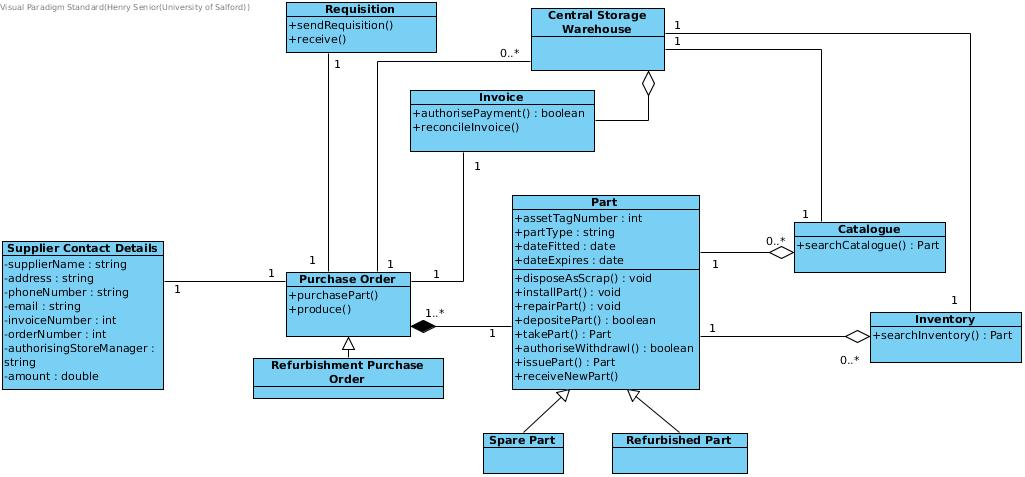
\includegraphics[width=21.5cm, angle=90, origin=h]{images/static-model.jpg}
\end{center}
\section{Activity Diagrams}
Activity Diagrams provide a way of combining the concepts of different UML modelling techniques. \cite{UML-Distilled} This makes them well suited to demonstrating how a system flows when completing different Use Cases.

\subsection{Activity Diagram 1: Purchase Parts}
\begin{center}
	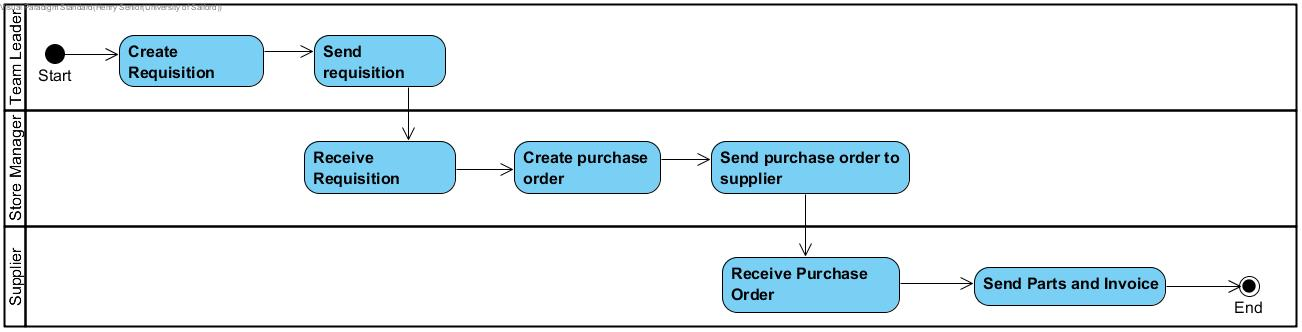
\includegraphics[width=\textwidth]{images/activity-diagram-1.jpg}
\end{center}

\subsection{Activity Diagram 2: Authorise Payments}
\begin{center}
	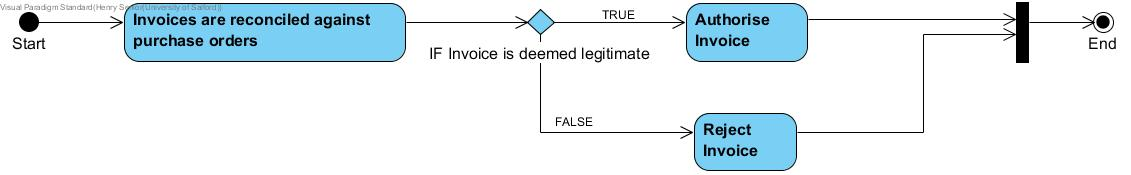
\includegraphics[width=\textwidth]{images/activity-diagram-2.jpg}
\end{center}

\section{Conclusion}
Through using UML, I found that it was possible to represent separate aspects of the system in different perspectives. By using modelling techniques such as a Use Case diagram, it was possible to show how different actors would interact with the system. However, as Use Cases do not represent individual components that make up the system, I soon found that I also required a Static Model. Whilst a Static Model will not show how the system is interacted with by users, it provides a clear and visual way of demonstrating how different modules within the system interact with one another. A Static Model also shows the relationships between the classes. In order to bring the Use Cases together with a Static Model, I chose to demonstrate how the system flows when in use with Activity Diagrams. Doing so joins together both the technical model of the system and the user focussed Use Cases. 
\\
By providing all three diagrams, the report provides a holistic overview of the power plant's central storage warehouse. This should allow other system designers to understand how the system would work and allow them to take the UML diagrams and implement the system as outlined in the scenario. 
\newpage
\bibliographystyle{agsm}
\begin{thebibliography}{9}
	\bibitem{UML-Distilled}
	Fowler M, Kendall S. 1999. UML Distilled: a brief guide to the standard object modelling language. 2nd Ed. Addison Wesley. 

	\bibitem{Lectures}
	Bass, J. 2017. Software Projects with Agile Techniques Lecture Notes. University of Salford
\end{thebibliography}

\end{document}          
